% (c) 2020 Stefan Antonowicz
% Based off of tex found at https://github.com/ludus-leonis/nipajin
% This file is released under Creative Commons Attribution-NonCommercial-ShareAlike 4.0 International License.
% Please do not apply other licenses one-way.

\renewcommand{\yggWitch}{%
  \mychapter{Witches}{witches}
}

\renewcommand{\yggWitchText}{%

  \mysection{Mojo}{witch-mojo}

  \mytable{X c r}{
    \thead{Level} & \thead{Mojo}\\
  }{
    1 & d8 \UD \\
    2-3 & d10 \UD \\
    4-5 & d12 \UD \\
    6-7 & d16 \UD \\
    8 & d20 \UD \\
    9 & d24 \UD \\
  }  

  Mojo is a \UD.  Mojo is used to cast \mylink{Charms}{witch-charms} and perform \mylink{Necromancy}{witch-necromancy}.

  When you cast Charms, you \RS your Mojo, once per Charm.  You can cast as many Charms as you like, as long as you have a Mojo \UD.

  When you perform Necromancy, you combine your Mojo \UD with your \FOC in a \RO attempt:

  \example {
    \mybold{Mojo Test}

    \RO : \mybold{Mojo \UD} plus \mybold{\FOC} plus \mybold{Modifiers}

  }

  Finally, you can use your Mojo \UD as if it were an Armor Die (see the Core Rules) if you fail your Guard \RO in Combat.

  \mysection{Cunning}{witch-cunning}

  Cunning is used to perform Occultism, and be used to help Spriggans create magic weapons.  A Cunning die is a d4; you have a base number of Cunning die equal to your \LVL (so if you were \LVL 6, you'd have 6d4 Cunning Dice).  You earn these Cunning Dice at the start of any Sabbatical you take.  Any Cunning Dice you do not use at the end of the Sabbatical are lost.

  You may obtain more Cunning Dice as specified below:

  \mytable{X X}{}
  {
    Wheel: Crown & +3 \\
    Wheel: Gibbous & +2 \\
    Wheel: Wax Quotidian & +1 \\
    Coven & +1 each member \\
    Familiar: & +1 if present \\
  }  


  You gain a Coven at 7th level (see Core Rules). 

  Cunning Dice can be traded be traded between you and other Witches. You can give as many Cunning Dice to different people as you wish, but you can only accept a number of Cunning Dice up to your \LVL-1.

  Each Occult rite requires 1 or more Cunning Dice to be rolled (how many is up to you).  You must obtain a number of successes (that is, roll a 3 or 4 on the Cunning Die) equal to or greater than what is specified in the Occult rite.  


 
  \mysection{The Wheel}{witch-the-wheel}

  Your Mojo moves counterclockwise through a Wheel of eight points - it ascends from the Void to Sickle, Quotidian, and Gibbous to Crown, then descends through Gibbous, Quotidian, and Sickle to return to the Void. 

  During character creation, roll a d8 to see where your Mojo begins:

  \mytable{l X}{}
  {
    1 & Void \\
    2 & Waning Sickle \\
    3 & Waning Quotidian \\
    4 & Waning Gibbous \\
    5 & Waxing Sickle \\
    6 & Waxing Quotidian \\
    7 & Waxing Gibbous \\
    8 & Crown \\
  }  

  Every Session, move your Mojo one step counter-clockwise along the wheel:
  \begin{center}
  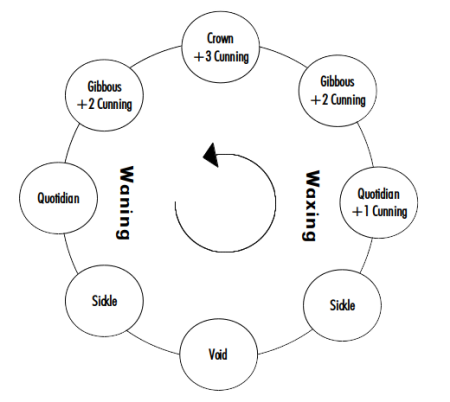
\includegraphics[scale=.3]{mojo_circle}
  \end{center}

  For some powerful rituals, you may need to move "[num] Widdershins" before you can attempt the ritual again.  A full Widdershins means you must make [num] transit(s) of the Wheel before you can cast the ritual again.  For example, if you were at Crown, you must travel to Waning Gibbous, then Waning Quotidian, etc. all the way back around to Crown before you can try again  (meaning you will need to play multiple Sessions).

  \newpage


\newpage


\mysection{Necromancy}{witch-necromancy}

You must \RO using your Mojo \UD plus your \FOC, in addition to the modifiers specified in the spell.  All Necromancy spells are considered part of the Death Paradigm, and not normally available to Sorcerers or Mystics.

\example {
  \mybold{Necromancy Roll}

  \RO : \mylink{Mojo}{witch-mojo} plus \FOC plus \mybold{Modifiers}
}



When a corpse is "consumed", it immediately evaporates into greasy black smoke.  The sound of a single screaming voice can be faintly heard.

Where the duration indicates "\LVL Minutes", the Arbiter will use a timer to measure the actual time.



\newpage



} %end
